% !TeX spellcheck = cs_CZ
%{\tikzset{external/prefix={tikz/FYZI/}}
% \tikzset{external/figure name/.add={ch54_}{}}
%---------------------------------------------------------------------------------------------------
% file history_AFYZ.tex
%---------------------------------------------------------------------------------------------------
%=============================== Kapitola: Astrofyzika =============================================
\chapter{Úvod}
\minitoc

  \wikiAstrofyzika  je vědní obor ležící na rozhraní \emph{fyziky} a \emph{astronomie}. Zabývá se 
  fyzikou vesmíru, včetně fyzikálních vlastností (svítivost, hustota, teplota, chemické složení) 
  astronomických objektů jako jsou hvězdy, galaxie a mezihvězdná hmota, jakož i jejich vzájemné 
  působení.
  
  Podle metod výzkumu těchto objektů se dělí na \emph{fotometrii}, \emph{spektroskopii},
  \emph{radioastronomii}, \emph{astrofyziku rentgenovou}, \emph{infračervenou}, 
  \emph{ultrafialovou} a \emph{neutrinovou}. Každý z těchto podoborů se dále dělí na praktickou a 
  teoretickou část. Praktická získává potřebná data. Teoretická s pomocí fyzikálních zákonů 
  vysvětluje pozorované cho\-vá\-ní vesmírných těles.
  
  \section{Historie astrofyziky}
  
  \section{Základní vztahy}
    \begin{itemize}
      \item \wikiAU - \emph{astronomická jednotka}: průměrná vzdálenost Země od Slunce, 
      $\SI{150e6}{\km}$. Vzájemné vzdálenosti planet či jiných objektů sluneční soustavy 
      vy\-já\-dře\-né v AU poskytují relativně názorné měřítko vzdáleností těchto objektů od sebe. 
      Přesná hodnota je
      \begin{equation*}
        \sisetup{separate-uncertainty}
        1 AU = \SI[multi-part-units = single]{149597870691(6)}{\m}
      \end{equation*}
      Kvůli vyšší přesnosti \emph{Mezinárodní astronomická unie} (International Astronomical 
      Union, IAU) přijala novou de\-fi\-ni\-ci, podle které je AU délka poloměru nerušené oběžné 
      kruhové dráhy tělesa se zanedbatelnou hmotností, pohybujícího se okolo Slunce rychlostí 
      \newline \(\num{0,017202098950}\) radiánů za den (\(\SI{86400}{\second}\)). 
        \begin{itemize}
          \item Vzdálenost Země od Slunce je \SI{1.00(2)}{\AU}.
          \item Měsíc obíhá kolem Země ve vzdálenosti\newline \SI{0,0026(1)}{\AU}.
          \item Mars je od Slunce vzdálen \SI{1.52(14)}{\AU}.
          \item Jupiter je od Slunce vzdálen \SI{5.20(5)}{\AU}.
          \item Nejvzdálenější člověkem vyrobené těleso, sonda \newline Voyager 1, bylo 31.
                prosince 2007 ve vzdálenosti \SI{104.93}{\AU} od Slunce.
          \item Průměr sluneční soustavy bez \emph{Oortova oblaku} je přibližně \SI{105}{\AU}.
          \item Průměr sluneční soustavy s Oortovým oblakem se odhaduje na \SI{50000}{\AU} až    
                \SI{100000}{\AU}.
          \item Nejbližší hvězda (po Slunci), \emph{Proxima Centauri}, se nachází přibližně ve 
                vzdálenosti \SI{268000}{\AU}.
          \item Průměr hvězdy Betelgeuze je \SI{2.57}{\AU}.
          \item Vzdálenost Slunce od středu Galaxie je přibližně \SI{1.7e9}{\AU}.
          \item Velikost viditelného vesmíru je asi \SI{8.66e14}{\AU}.
        \end{itemize}
      \item \textbf{\si{\lightyear}} - \emph{světelný rok}: vzdálenost, kterou světlo ulétna za    
            jeden rok, \SI{9.46e12}{\km},
      \item \textbf{\si{\parsec}} - \emph{parsek, paralaktická sekunda}: vzdálenost, ze které by  
            poloměr oběžné dráhy Země byl kolmo k zornému paprsku vidět pod úhlem 
            \SI{1}{\arcsecond}, 
            \SI{30.9e12}{\km}. 
    \end{itemize}
    
    %---------------------------------------------------------------
    % !TeX spellcheck = cs_CZ
\wikitextrule
\begin{example}\label{FYZ:exam005}
  Spočtěte, jakou vzdálenost v metrech vyjadřuje jeden parsek \protect\cite[s.~3]{Kulhanek2009}.
  
  \textbf{Řešení}: \(\SI{1}{\parsec}\) (paralaktická sekunda) je vzdálenost, ze které vidíme 
  velkou poloosu oběžné dráhy Země kolem Slunce pod uhlem \(\varphi = \ang{;;1}\). Úhel 
  \(\ang{;;1}\) je tak malý, že strany \(VS\) a \(VZ\) na obrázku prakticky splývají a místo 
  pravého trojúhelníka $VSZ$ můžeme použít definiční vztah úhlu v obloukové míře (\emph{velkost 
  úhlu je možné určit jako poměr délky oblouku vymezeného rameny na kružnici opsané kolem 
  vrcholu k poloměru této kružnice}). Proto 
  
   {\centering
    \captionsetup{type=figure}
    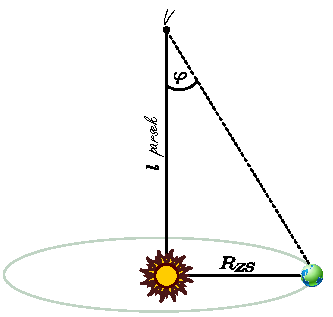
\includegraphics[width=0.6\linewidth]{fyz_fig224.pdf}
    \captionof{figure}[Parsek]{K příkladu \ref{FYZ:exam005}: Odvození velikosti Parseku}
    \label{fyz:fig224}
    \par}
  \begin{equation*}
    \varphi = \frac{R_{SZ}}{l} \rightarrow l = \frac{R_{SZ}}{\varphi},
  \end{equation*}
  kde $l$ je vzdálenost \SI{1}{\parsec} v metrech, $R_{SZ}$ je vzdálenost země od Slunce a 
  $\varphi$ je úhel jedné vteřiny vyjádřený v radiánech. 
  \begin{equation*}
      l = \frac{\SI{1.5e11}{\meter}}{\dfrac{1}{60\cdot60} 
          \cdot\dfrac{2\pi}{360}}\cong \SI{3e16}{\meter}.
  \end{equation*}
\end{example}
\wikitextrule
    %---------------------------------------------------------------
    Další jednotkou, kterou se v astrofyzice měří vzdálenost dvou vesmírných těles, je 
    \emph{paralaxa}. Pozorovací místa musí být od sebe výrazně vzdálena, aby například při měření 
    vzdálenosti naší nejbližší hvězdy - \emph{Proxima Centauri} byla paralaxa vůbec měřitelná. 
    Vzdálenost této hvězdy je \num{4.2} světelných let (nebo \SI{270000}{\AU}) od Země.
     
    %---------------------------------------------------------------
    % !TeX spellcheck = cs_CZ
\wikitextrule
\begin{example}\label{FYZ:exam006}
  Najděte paralaxu Proximy Centauri, která je od nás vzdálená asi \num{4.2} světelného roku 
  \protect\cite[s.~4]{Kulhanek2009}.
  
   {\centering
    \captionsetup{type=figure}
    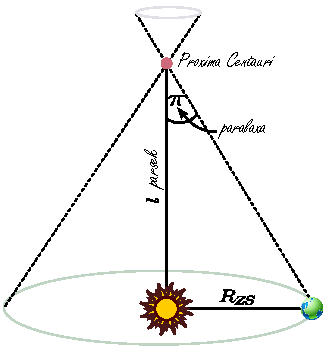
\includegraphics[width=0.8\linewidth]{fyz_fig225.pdf}
    \captionof{figure}{K příkladu \ref{FYZ:exam006}: Paralaxa naší nejbližší hvězdy}
    \label{fyz:fig225}
    \par}
    
  \textbf{Řešení}: Díky pohybu Země kolem Slunce se zdá, že blízké hvězdy opisují oproti 
  vzdáleným elipsu. Úhlový poloměr této elipsy se nazývá paralaxa hvězdy. Lze ji změřit jen pro 
  nejbližší hvězdy. Z definice úhlu (jako v předchozím příkladě) tedy vyplývá, že
  \begin{equation*}
    \pi = \frac{R_{ZS}}{l} = \frac{\SI{1.5e11}{\meter}}{\SI{4.2}{\lightyear}} 
        = \frac{\SI{1.5e11}{\meter}}{\num{4,2}\cdot\SI{9.5e15}{\meter}}
          \cong \SI{3,7e-6}{\radian},
  \end{equation*}
  
  což je přibližně \(\ang{;;0,76}\). Vidíme, že i u druhé nejbližší hvězdy po Slunci není 
  paralaxa ani celá \(\ang{;;1}\).
\end{example}
\wikitextrule
    %---------------------------------------------------------------

%} %tikzset
---------------------------------------------------------------------------------------------------
\printbibliography[title={Seznam literatury},heading=subbibliography]
\addcontentsline{toc}{section}{Seznam literatury}